\chapter{Influence du feedback stellaire sur les propriétés des galaxies dans les simulations de la Réionisation}
\label{sec:galaxies}

%\subsubsection{Impact sur la fraction d'ionisation}
%\label{sec:pbfesc}

Une observation importante par rapport aux tests de la section \ref{sec:testsncosmo} est qu’indépendamment de la quantité d'énergie injectée l'histoire d'ionisation reste quasiment inchangée (cf figure \ref{fig:xion_sneff}), alors que le \ac{SFR} est significativement impacté.
Cet effet est inattendu car si la quantité d'étoiles diminue, la quantité de radiation diminue d'autant, et donc la fonction d'ionisation globale devrait être impactée.
%Or ce n'est pas ce qui est observé ici.
Dans le but d'explorer cet effet, nous allons nous concentrer dans cette section sur une étude galaxies par galaxies.

\begin{figure}
        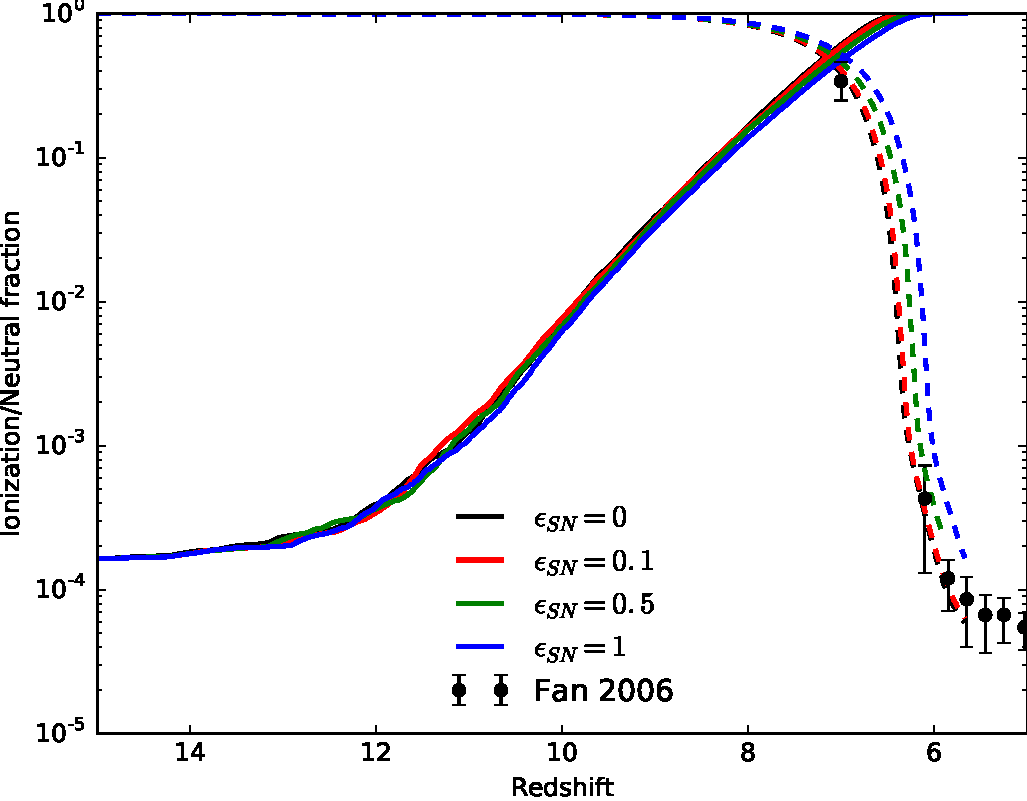
\includegraphics[width=.95\textwidth]{img/03/sneff_xion.pdf} 
        \caption[Fonction d'ionisation en fonction de la quantité d'énergie injectée]{Malgré une SFH différente (voir figure \ref{fig:sfr_egy}), l'histoire d'ionisation est conservée en changeant la quantité d'énergie injectée.
        }
 		\label{fig:xion_sneff}
\end{figure}

%\section{La détection des halos}

%Les étoiles se forment rarement de manière isolée mais généralement en groupe, dans des régions bien définies. % que l'on nomme galaxies.
%Ces zones ont une densité de gaz particulièrement élevée qui leurs permettent d'amorcer la formation stellaire. %et disposent donc de suffisamment de matériaux pour amorcer
%Comme la densité de gaz suit la distribution de matière noire, c'est grâce à cette dernière que l'on détecte les galaxies.
%L'idée est d'utiliser un "détecteur de halo" (ou "halo finder") pour détecter les surdensités de matière noire, auquel on cherchera ensuite à associer la composante baryonique qui compose les galaxies.


Cette partie a pour objectif de présenter les méthodes de détection des galaxies, pour pouvoir ensuite mener une série d'études statistiques.
Nous analyserons différentes propriétés des galaxies en fonction de la masse de leur halo hôte et nous nous intéresserons à des propriétés telle que la fraction de masse baryonique, le taux de formation stellaire, le taux d'éjection de matière en fonction des supernovæ, ou encore la fraction d'échappement du rayonnement.
%La comparaison de ces grandeurs en fonction du modèle de supernovae permettra de mettre en évidence

%L'étude des simulation se fait souvent halos par halos.
%Quand on cherche a déterminer es propriétés des galaxies, un paramètre important est leur masse.
%Comme le gaz suit la dynamique des baryons, les galaxies sont situées dans les surdensités de matière noire.



\section{Association halos - galaxies}



%Comme nous l'avons vu plus tôt (voir sec \ref{sec:solverDM}), le champ de matière noire utilise une représentation sous forme de particules.
%L'objectif d'un halo finder est de détecter les surdensités dans ce champs de particule.

Avant de pouvoir analyser les galaxies,il faut les détecter.
Les galaxies étant situées au sein de halos de matière noire, on détectera les halos dans une premier temps, puis on y associera la partie baryonique représentant les galaxies.

Pour la détection des halos, j'ai principalement utilisé l’algorithme \ac{FOF} et plus particulièrement \textit{pFOF} une de ses implémentations parallèle. % \citep{2014A&A...564A..13R}.
\textit{pFOF} lie les particules regroupées en surdensité, en cherchant de proche en proche les particules à une distance inférieure à une taille de lien caractéristique.
Il retourne ensuite une liste de groupes de particules et une liste de positions déterminées par le centre de masse des particules de chaque halos.
%FOF retourne une liste de position de halo, une liste permettant de lier les particules détecté aux halos.
%Il existe plusieurs possibilités pour ensuite déterminer l'étendue spatiale des halos.
J'ai utilisé un paramètre de taille caractéristique de valeur standard $0,2$.


\subsection{Association dans le R$_{200}$}

La façon la plus directe pour déterminer l'étendue spatiale d'un halo consiste à utiliser l'approximation du $R_{200}$ \citep{1997ApJ...490..493N}.
Elle consiste à considérer, autour du centre de masse, une sphère aillant une densité moyenne de $200$ fois la densité moyenne de l'univers $\bar{\rho}$.
Le $R_{200}$ est défini comme : 
\begin{equation}
R_{200}= \left( \frac{3}{4\pi} \frac{M_{FoF} }{200 \bar{\rho}}  \right)^{1/3}
\end{equation}


%Il faut ensuite y associer les autres champs physique contenus par la grille 
%La première méthode consiste a utiliser l'approximation du R200.
%Il faudra associer, la matière noire, le gaz et les étoiles compris a l'intérieur d'une sphere de rayon R200.

%Il faut ensuite y associer les autres champs physique contenus par la grille 

%Le méthode est la suivante:
%
%\begin{itemize}
%\item générer un KDtree sur les particule de matière noire / les étoiles / la grille AMR
%\item Faire une recherche sphérique autour de la positions des halo, sur un rayon de R200
%\item stocker les indices dans une structure
%\end{itemize}

Nous avons à ce stade une position et une étendue pour chaque halo.
On cherchera ensuite à y associer les baryons formant les galaxies.
Pour se faire j'ai utilisé un KD-tree, un arbre permettant d'effectuer des recherches spatiales de manière optimisées.
A l'aide d'un arbre généré sur les étoiles, j'ai associé à chaque halo toutes les étoiles à une distance inférieur à son $R_{200}$ autour de son centre de masse.
Comme il est également intéressant d'obtenir des informations sur les champs physique contenus dans la grille \ac{AMR}, il sera possible d'utiliser un KD-tree sur la grille pour déterminer quelles sont les cellules qui se trouvent dans le $R_{200}$ du halo.
Il suffit pour cela de générer un arbre sur les centres des cellules à la place de la position des étoiles.
%Comme les particules de matière noire  données par FoF ne represente pas le meme volume, dans un soucis de cohérence, on appliquera cette méthodes a la matière noire également.
À ce stade nous avons donc la possibilité, pour chaque halo, de connaître toutes les grandeurs physiques comprissent dans son $R_{200}$.

\subsection{Le problème de la forme des halos}

%Fortement non viriallisé a z=6\\
%beaucoup de dynamique et merger dans les filemments

L'approximation du $R_{200}$ est valide et a fait ses preuves dans le cas de halos virialisés.  %TODO ref
Cependant, à haut redshift (z>5) les halos sont encore en formation et peuvent na pas être virialisé.
Il devient alors difficile pour \ac{FOF} de séparer les différentes sous-parties d'une même sur-densité.
La figure \ref{fig:part_halo} illustre particulièrement bien ce problème de détection.
Dans ce cas, la sur-densité détectées par \ac{FOF} est loin d'être sphérique, et l'approximation du $R_{200}$ n'est pas valide.
Du fait de l'effondrement hiérarchique de la matière noire, changer la longueur de lissage ne changera pas le problème et ne ferait que le reporter à d'autres échelles.

\begin{figure}
	\centering
	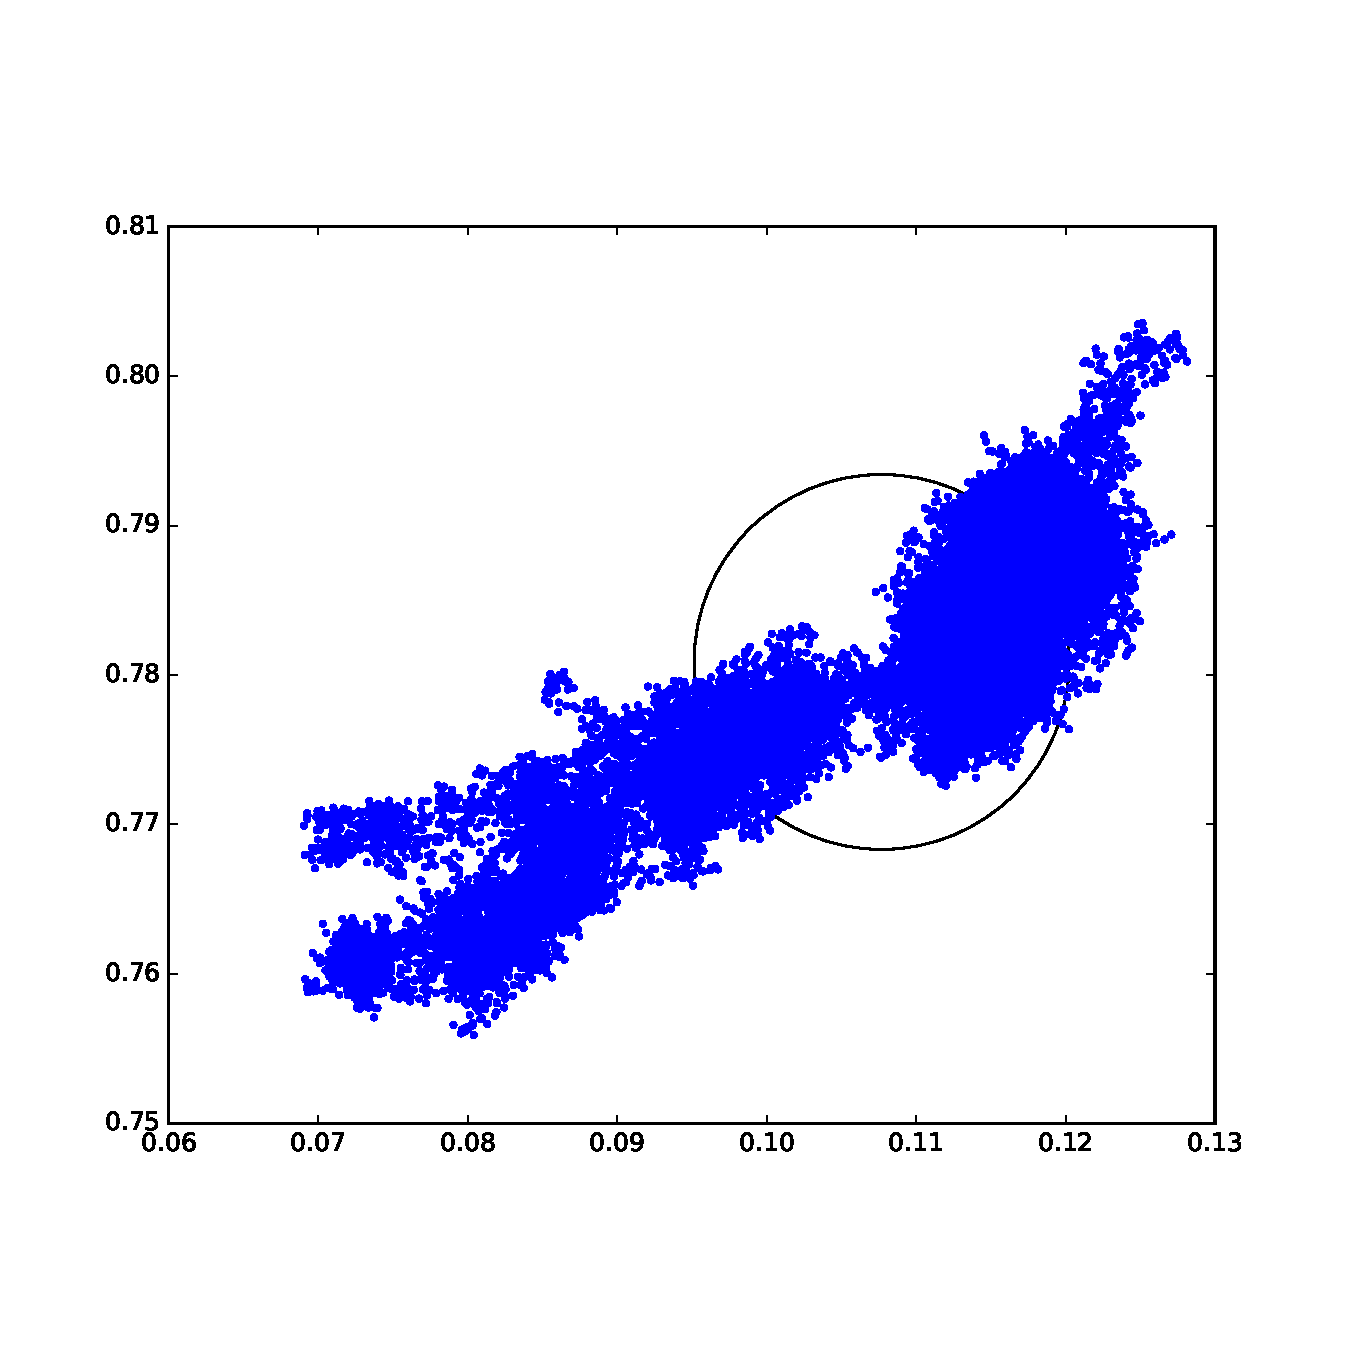
\includegraphics[width=.65\textwidth]{img/03/part_halo_R200.pdf} 
    \caption[Détection des halos]{La détection des halos par \ac{FOF} peux être difficile à haut redshift car les structure peuvent ne pas être virialisée.
    Les points bleus représentent les particules de matière noire et le cercle le $R_{200}$.
 	\label{fig:part_halo}}
\end{figure}


\subsection{Association "fine"}

Dans le but d'améliorer ces problèmes d'association avec la grille dans les halos les plus massifs pouvant être fortement asphériques, j'ai développé une méthode consistant a calculer l'intersection entre la grille et les particules du halos.
%pour associer plus précisément la grille aux halos.
Cette méthode consiste à rechercher pour chaque particule de matière noire, sa plus proche cellule.

La figure \ref{fig:R200_fine} présente la comparaisons entre la détection des cellules par $R_{200}$ et la méthode fine, pour le halo de la figure \ref{fig:part_halo}.
La méthode fine associe la grille de manière bien plus précise que la méthode $R_{200}$.
Malgré la recherche effectué à l'aide d'un KD-tree, cette méthode est évidemment bien plus longue qu'une simple recherche dans la sphere.

\begin{figure}
	\subfloat[$R_{200}$]{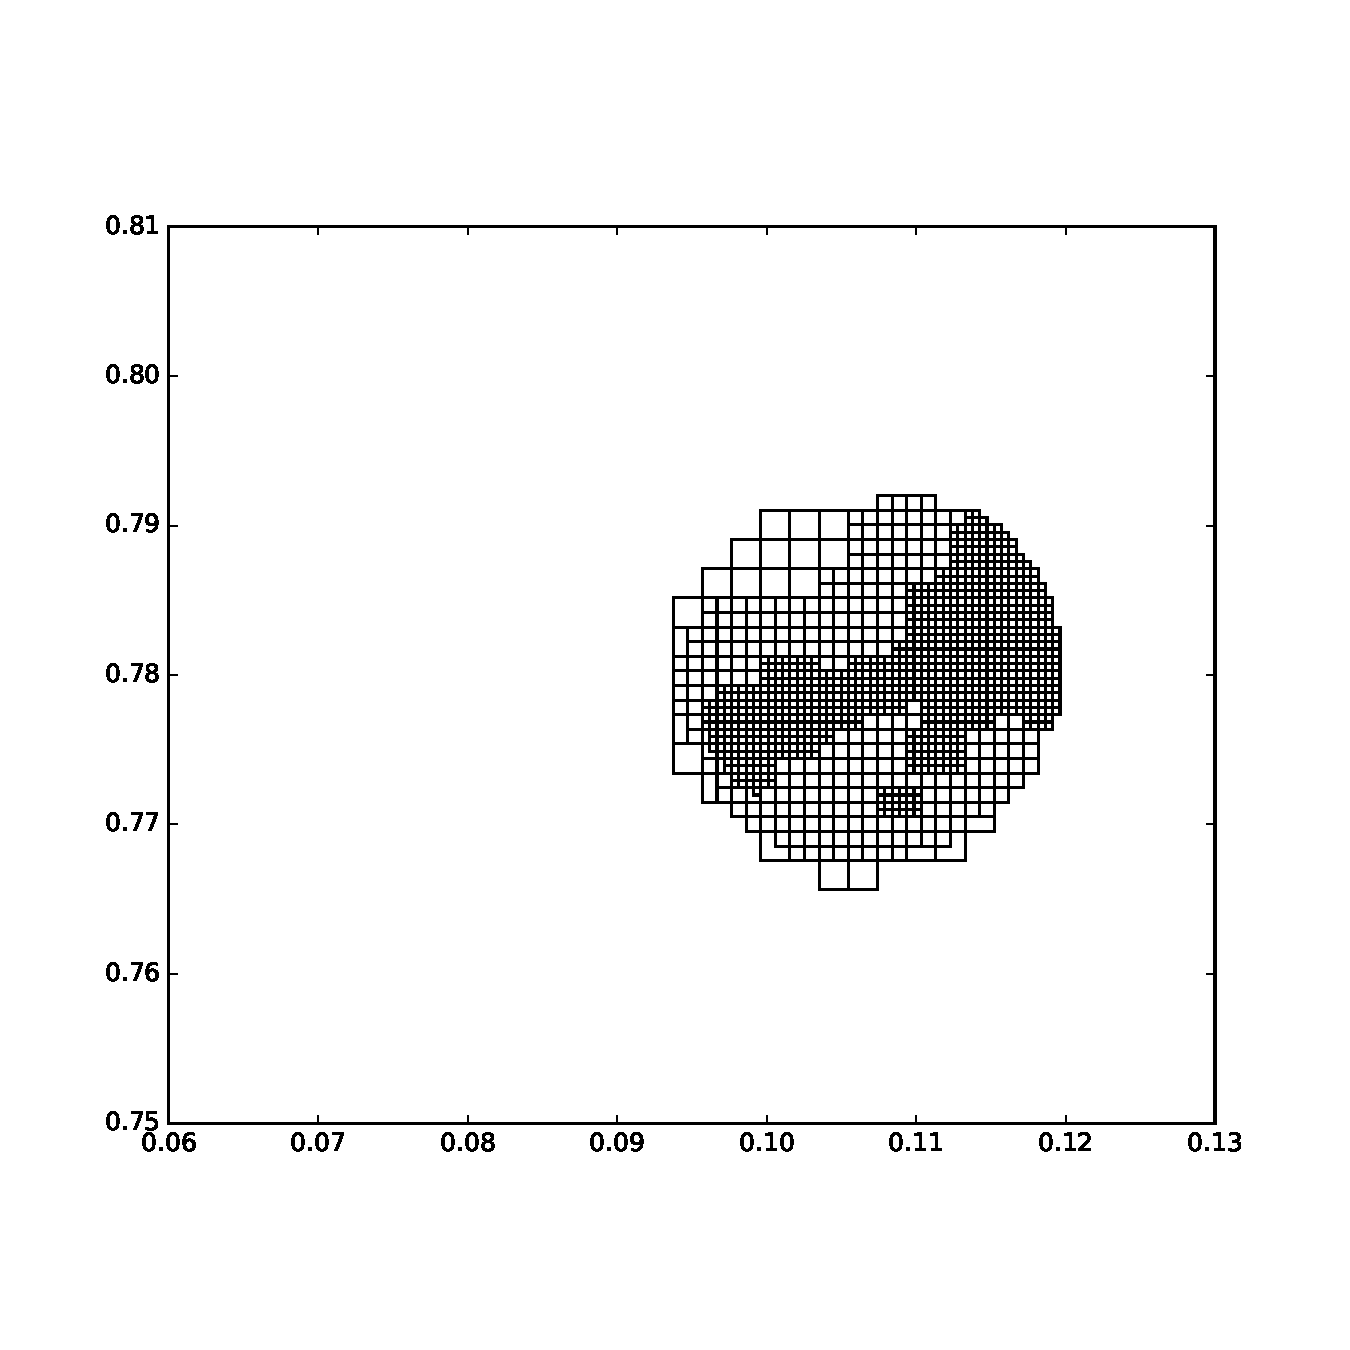
\includegraphics[width=.5\linewidth]{img/03/part_cells.pdf} }
	\subfloat[\textit{fine}]{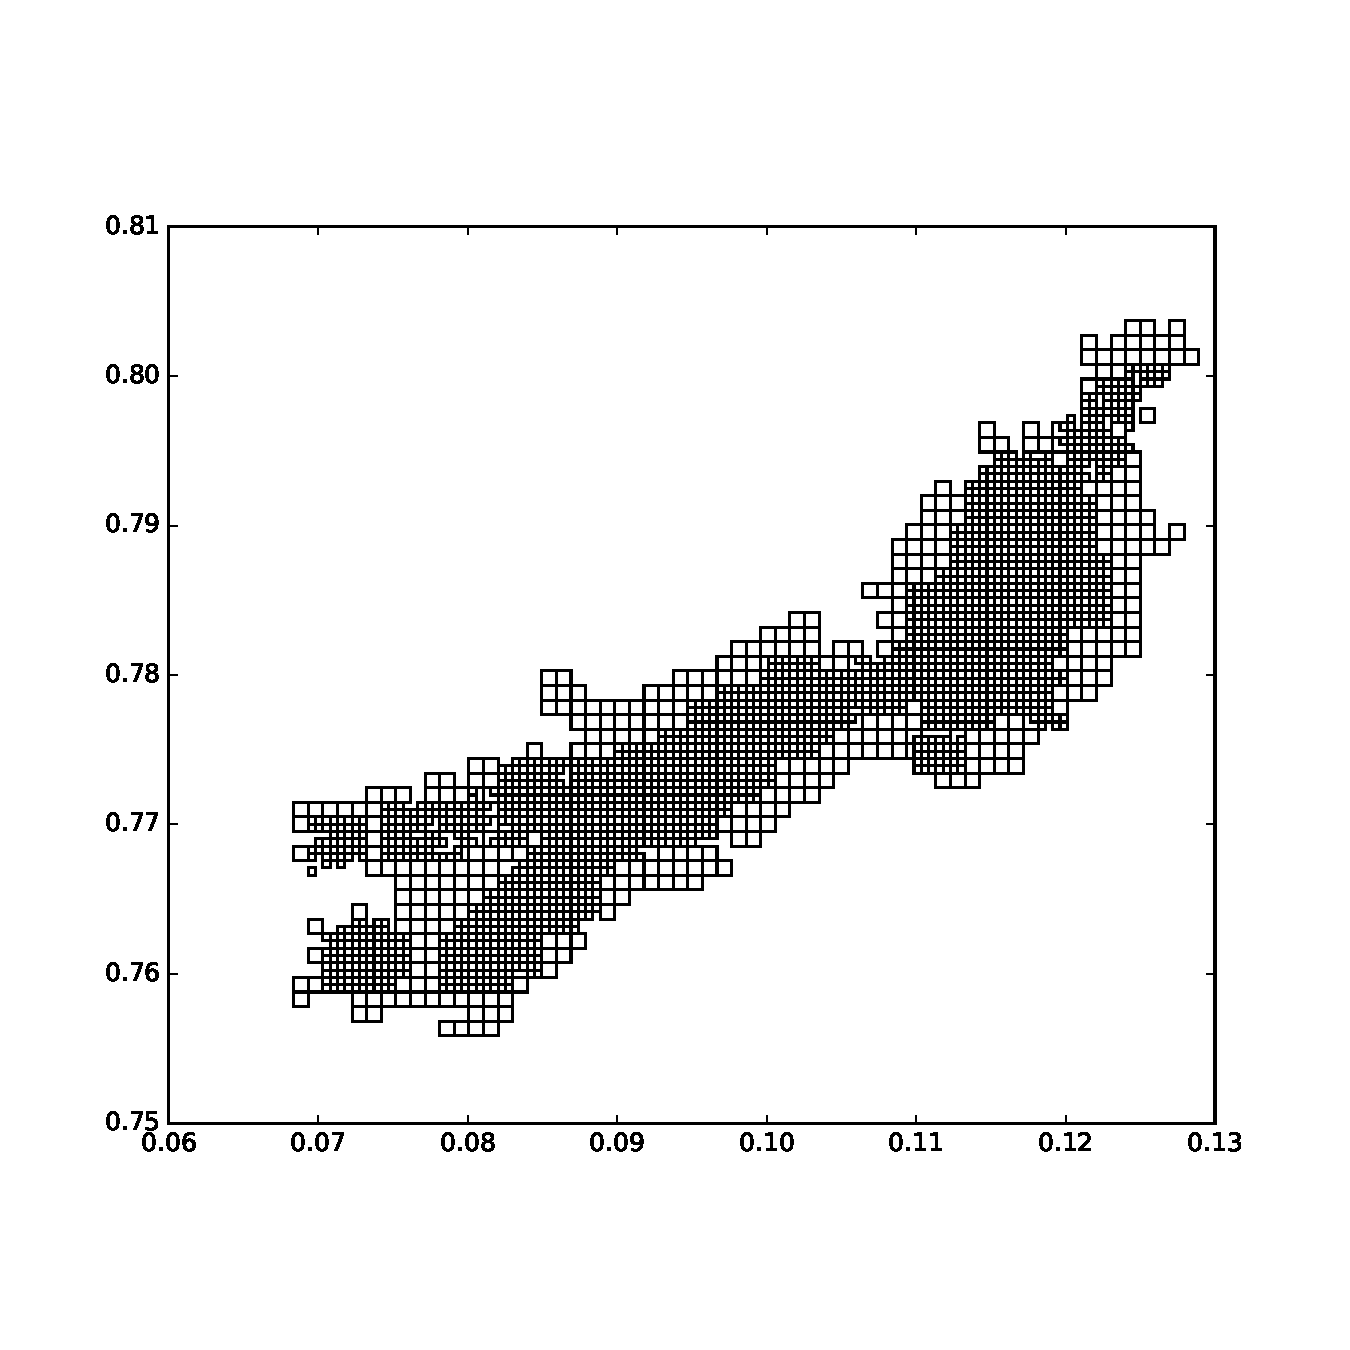
\includegraphics[width=.5\linewidth]{img/03/part_cells_fine.pdf} }
    \caption[Méthodes d'association matière noire - grille]{Cellules associées au halo présenté sur la figure \ref{fig:part_halo} dans le cas de l'estimation du $R_{200}$ à gauche et dans le cas de la méthode "fine" à droite.
    Ce halo étant fortement asphérique, l'approximation du $R_{200}$ est peu représentative.
    La méthode "fine" respecte mieux les contours et améliore significativement l'association halos-grille.
 	\label{fig:R200_fine}}
\end{figure}

\subsection{Association des petits halos}

Pour les petits halos, peu résolus, la taille des cellules peut être grandes par rapport au $R_{200}$.
Pour minimiser l'erreur commise, il est nécessaire d’estimer l'intersection entre le cube de la cellule et la sphère du halo.
J'ai résolu ce problème géométrique en projetant la grille \ac{AMR} sur une grille régulière de résolution arbitraire.
Cette méthode permettra d'associer des sous parties de cellules aux halos en approximant l'intersection avec la cellule et améliorera la precision globale de l'association (cf figure \ref{fig:intersec}).

\begin{figure}
	\centering
	%TODO refaire cette image
	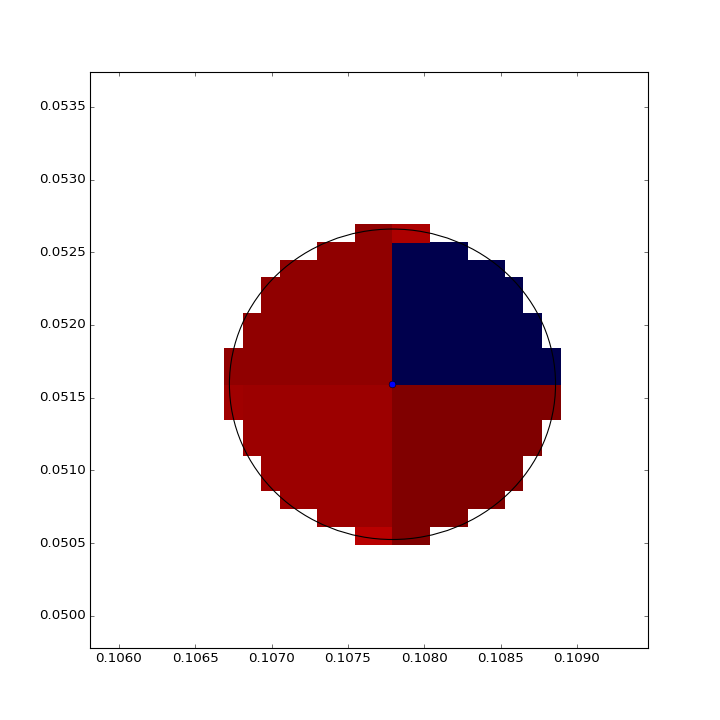
\includegraphics[width=.4\linewidth]{img/03/intersec.png}
    \caption[Projection des petits halo]{Les plus petits halos peuvent avoir des tailles comparable aux cellules.
    Il est nécessaire d’estimer l'intersection cube/sphère.
 	\label{fig:intersec}}
\end{figure}

\clearpage
\section{Étude de la composition des halos en fonction du feedback de supernovae}

A ce stade, nous avons définis la position et la taille de tous les halos et définis les galaxies par associations.
%Maintenant que nous pouvons associer toutes la physique au sein de chaque halo, 
Nous pouvons étudier l'influence du feedback de supernovae sur différentes caractéristiques des galaxies.
%différentes caractéristiques en fonction du type de feedback.
Les simulations analysées ici sont celles de la section \ref{sec:snmethod}.

\subsection{Approche visuelle}
\label{sec:snmaps}

Et première approche du problème, j'ai réalisé des cartes de champs, et simplement comparé visuellement la forme de quelques halos entre les simulations.
La figure \ref{fig:halo} présente le halo le plus massif ($M\approx10^{11} M_\odot$) extrait des trois simulations avec rayonnement (cf section \ref{sec:SNmodel}).
On y observe que le modèle cinétique est capable de générer des bulles de gaz chaud significativement plus grandes que dans le cas du modèle thermique.
De plus on observe dans la densité des coquilles dues aux vents générés, autour du halo central dans le cas du modèle cinétique.

\begin{figure}
		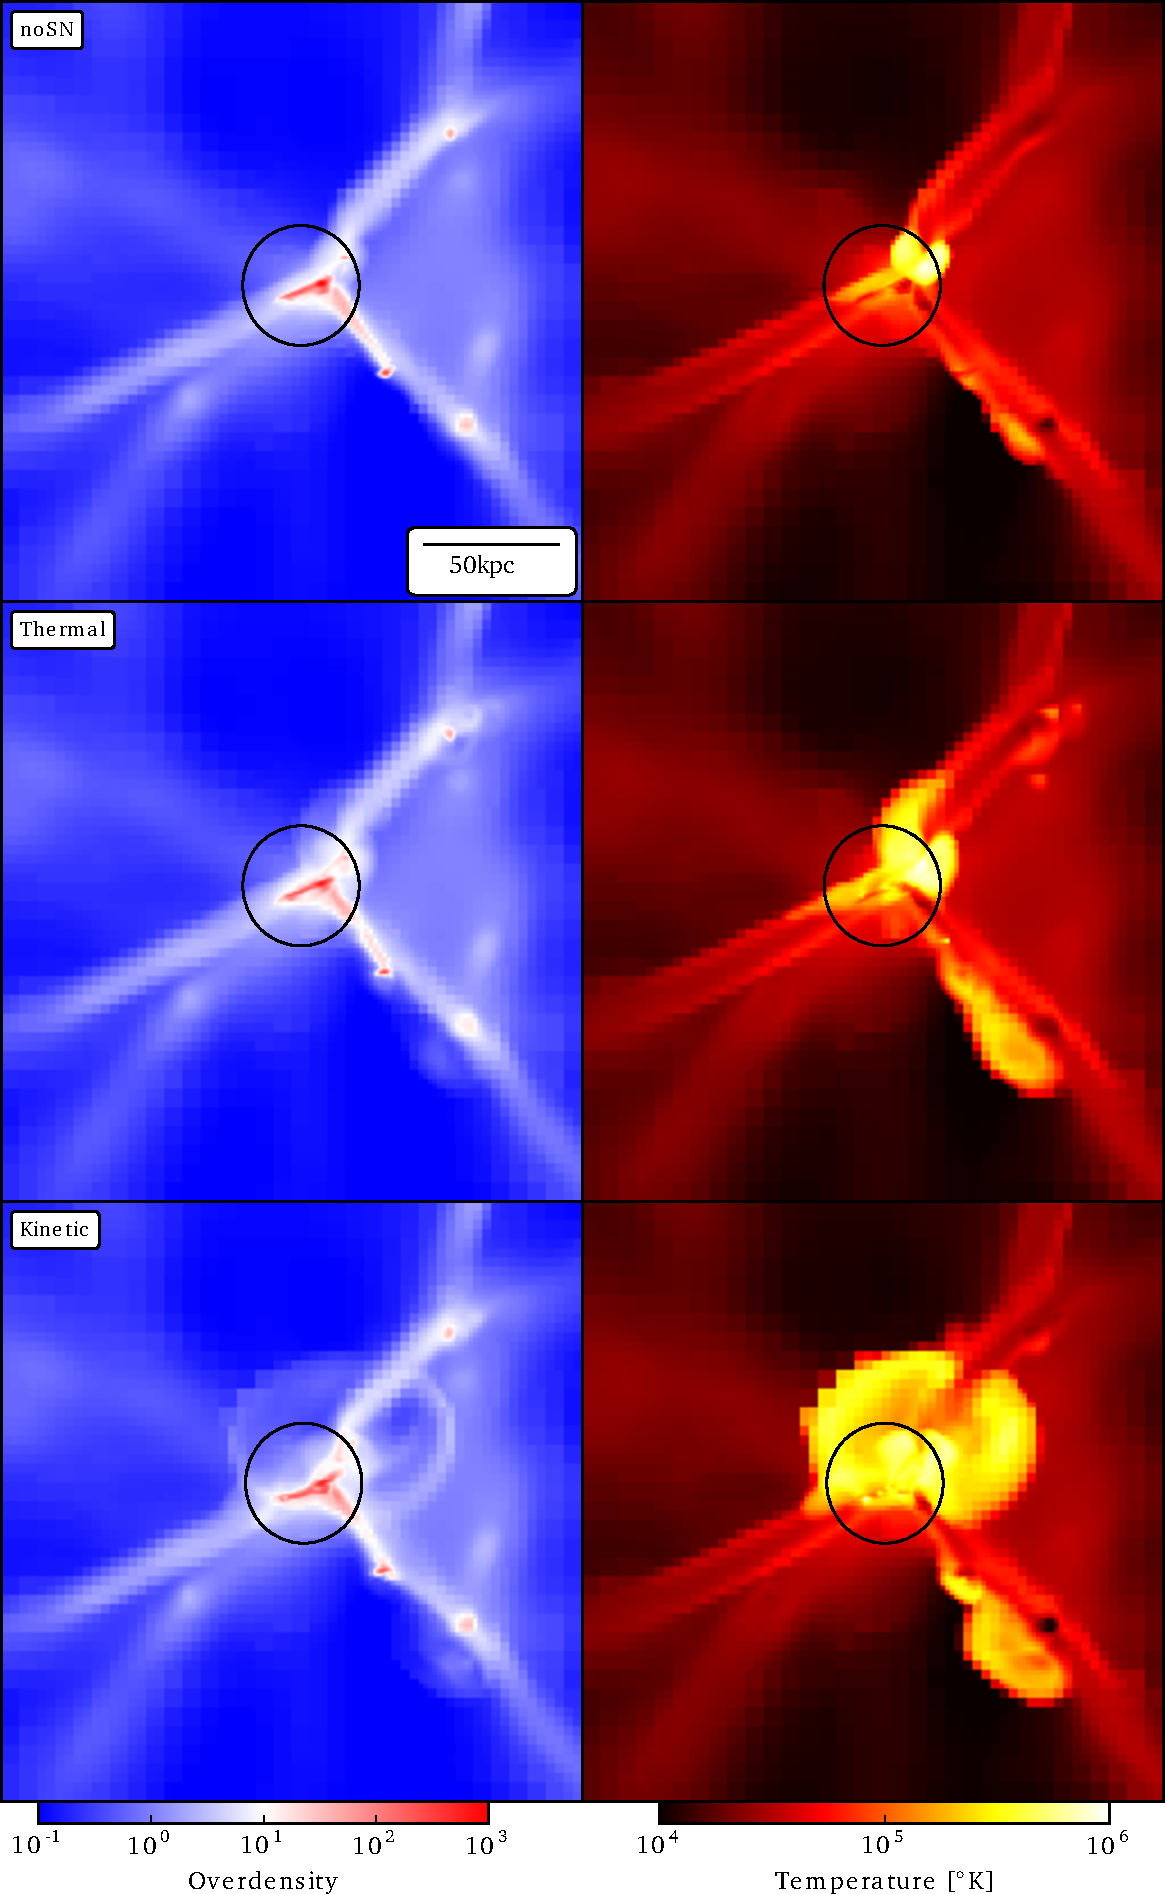
\includegraphics[width=.95\linewidth]{img/03/halos.pdf}
        \caption[Influence du modèle de supernovae sur la forme des halos]{Influence du modèle de supernovae sur la distribution de densité et de température d'un halo.
        Le cercle représente le $R_{200}$.
        Le modèle cinétique permet la création de vents formant des coquilles autour du halo, et la région chaude est bien plus large que dans le cas du modèle thermique.
 		\label{fig:halo}}
\end{figure}


\subsection{Les fonctions de masse}
\label{sec:hmf}

Sur la figure \ref{fig:ghmf} sont présentées les \ac{HMF}, représentées ici en cumulative (n>M) et comparées à un modèle analytique \citep{1999MNRAS.308..119S}.
%Le calcul de la \ac{GMF} ne considère que la masse des étoiles et non la totalité de la masse baryonique.
On observe un léger décrochage de la \ac{HMF} pour les plus petits halos ( $M< \mathrm{qq} 10^8 M_\odot$), mais celle ci n'est pas impactée par le feedback de supernovae dans nos modèles.
%A l'inverse, la \ac{GMF} est significativement réduite avec le feedback.
%On observe encore ici que le modèle de feedback cinétique a plus d'influence que le modèle thermique.

\begin{figure}
		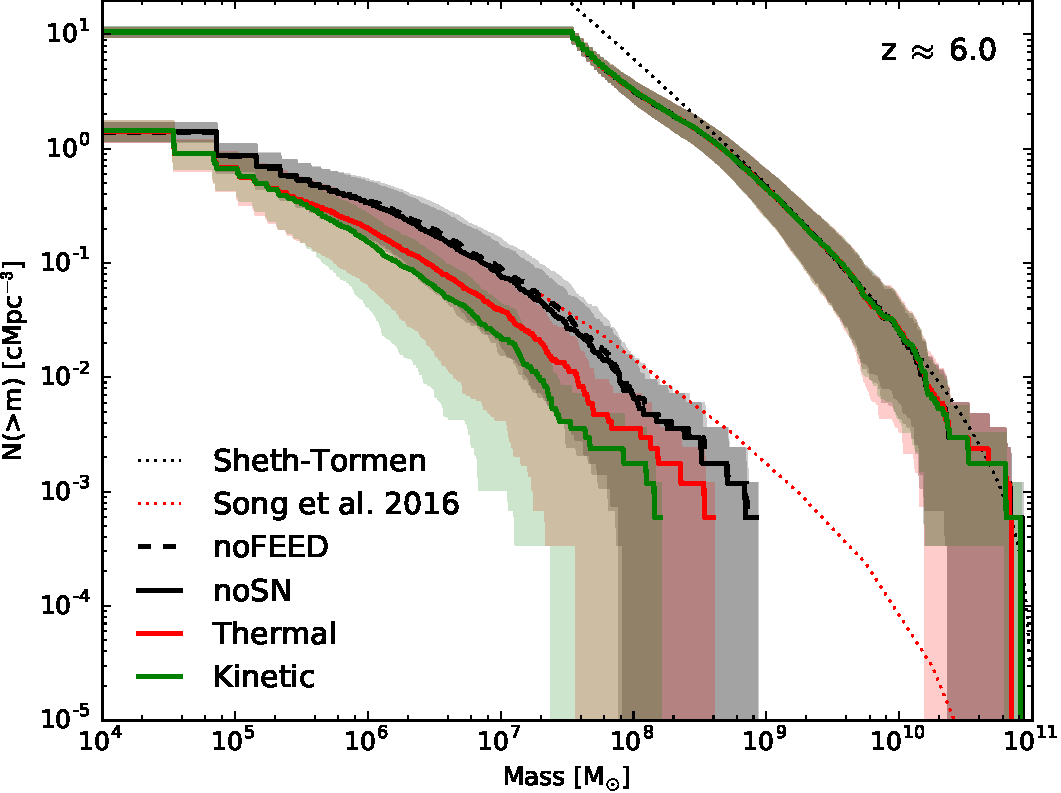
\includegraphics[width=.95\linewidth]{img/03/ghmf.pdf}
        \caption[Fonctions de masses des halos]{Fonction de masse des halos (\ac{HMF}) pour différents type de feedback de supernovae.
        Le feedback n'a pas d'influence directe sur la function de masse des halos
 		\label{fig:ghmf}}
\end{figure}

%\subsection{La masse d'étoiles en fonction de la masse du halo}
%Plus un halo est massif, plus celui ci va contenir d'étoiles.


\subsection{La formation stellaire en fonction de la masse du halo}
\label{sec:sfr_halo}
Connaissant, à un instant donné, les étoiles appartenant à chaque halo, il est possible de connaître leurs ages, et donc de déterminer l'histoire de formation stellaire de tous les halos.
%Nous allons voir que la masse 
%Il existe deux facons de voir 
Nous nous intéressons ici au \ac{SFR} à redshift $z=6$.
Comme il n'est pas possible de déterminer un taux instantané, le calcul sera réalisé sur les étoiles apparues dans une période de 10 Myrs.
Le \ac{SFR} d'un halo est défini comme :
\begin{equation}
	SFR_{10}^{halo} = \frac{ \sum M_{\star} \left( r<R_{200}^{halo}; t<10\mathrm{Myr}\right) }{10\mathrm{Myr}}.
\end{equation}
La formation stellaire peux être analysée de deux façons.
Dans un cas l'objectif est de déterminer la \ac{SFR} moyenne d'un halo en fonction de sa masse, dans l'autre on cherche à mesurer la contribution d'une classe de masse donnée à la \ac{SFR} globale.
Le lien entre les deux, n'est autre que la \ac{HMF} présentée à la section \ref{sec:hmf}.
Les résultats obtenus sont présentés sur la figure \ref{fig:sfr_halo}.
On observe que pour le feedback cinétique, la \ac{SFR} moyenne est réduite pour les halos les plus lourd, ce qui n'est pas le cas pour le feedback thermique où la \ac{SFR} a tendance à être réduite pour les petites masses de halos.
Sur les courbes de \ac{SFR} totale, on observe que les halos de masses $M\approx10^{10}M_\odot$ contribuent le plus à la formation stellaire dans ces simulations.
On remarquera également que la chute de \ac{SFR} n'est pas franche, et est en faveur d'un problème de non convergence dans la taille des simulations.
Si la \ac{HMF} était suffisamment échantillonnée au hautes masses, elle chuterait assez rapidement pour couper la \ac{SFR} cumulée des halos les plus massifs.
Ces simulations présentent donc une manque au niveau des sources de photons les plus intenses.

\begin{figure}
		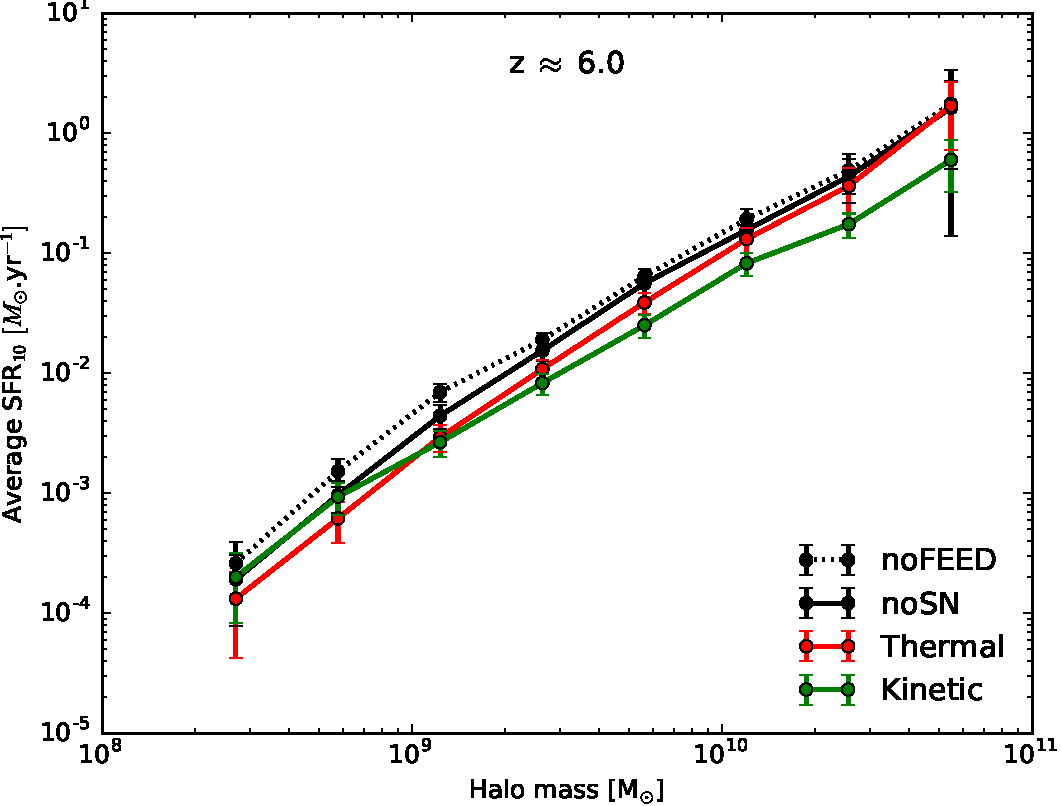
\includegraphics[width=.95\linewidth]{img/03/SFR_halo_avg.pdf}
		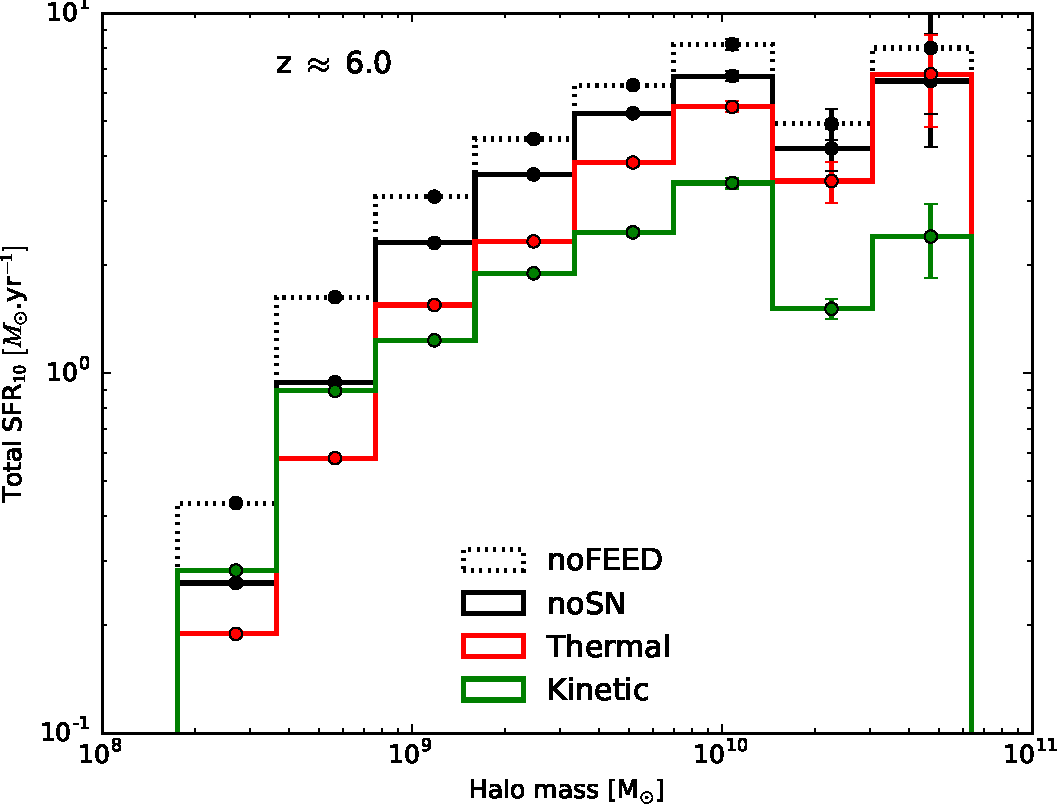
\includegraphics[width=.95\linewidth]{img/03/SFR_halo_tot.pdf}
        \caption[SFR en fonction de la masse du halo]{SFR en fonction de la masse du halo moyenne en haut et total en bas.
        }
 		\label{fig:sfr_halo}
\end{figure}



\subsection{La fraction baryonique}
\label{sec:baryon_frac}

La fraction baryonique est une grandeur essentielle pour caractériser un halo.
En effet, les baryons sont responsable de la formation stellaire, et donc de l'apparition des sources de rayonnement.
De plus, le rayonnement n'interagit qu'avec les baryons : plus un halo aura de baryon, plus le rayonnement aura de difficultés à s'en échapper.
La fraction baryonique est définie comme étant le rapport de la masse de baryon contenue dans un halo sur la masse totale de ce halo : 
\begin{equation}
f_b = \frac{M_* + M_{gas} }{M_{DM} + M_* + M_{gas} }
\end{equation}
La figure \ref{fig:bfrac} présente les résultats obtenus en unité de fraction baryonique universelle : $U_{bf}= \Omega_b/\Omega_m \approx 0,15$.
L'association fine est utilisée.
Sans feedback, les halos les plus massifs ont une fraction baryonique qui tend vers la fraction baryonique universelle.
On observe une décroissance de la fraction baryonique avec le feedback.
Cette décroissance est particulièrement marquée pour les halos les plus massifs avec le feedback cinétique.
Comme nous avons vu (section \ref{sec:hmf}) que la \ac{HMF} n'est pas impactée par le feedback, la diminution de la fraction baryonique observée ici est en fait une diminution de la quantité de baryon dans les halos.
Les baryons sont expulsés hors des halos par le feedback.
Cette décroissance peux être liée à celle observée sur la figure \ref{fig:sfr_halo}.
La \ac{SFR} est réduite car les baryons sont expulsés par le feedback.

%TODO parler de la résolution en masse pour les petites masses


%La résolution des halos les moins massifs est limitée, en masse,  en espace, en formation stellaire et en radiation.
%Les petits halo c'est de la MERDE!

\begin{figure}
		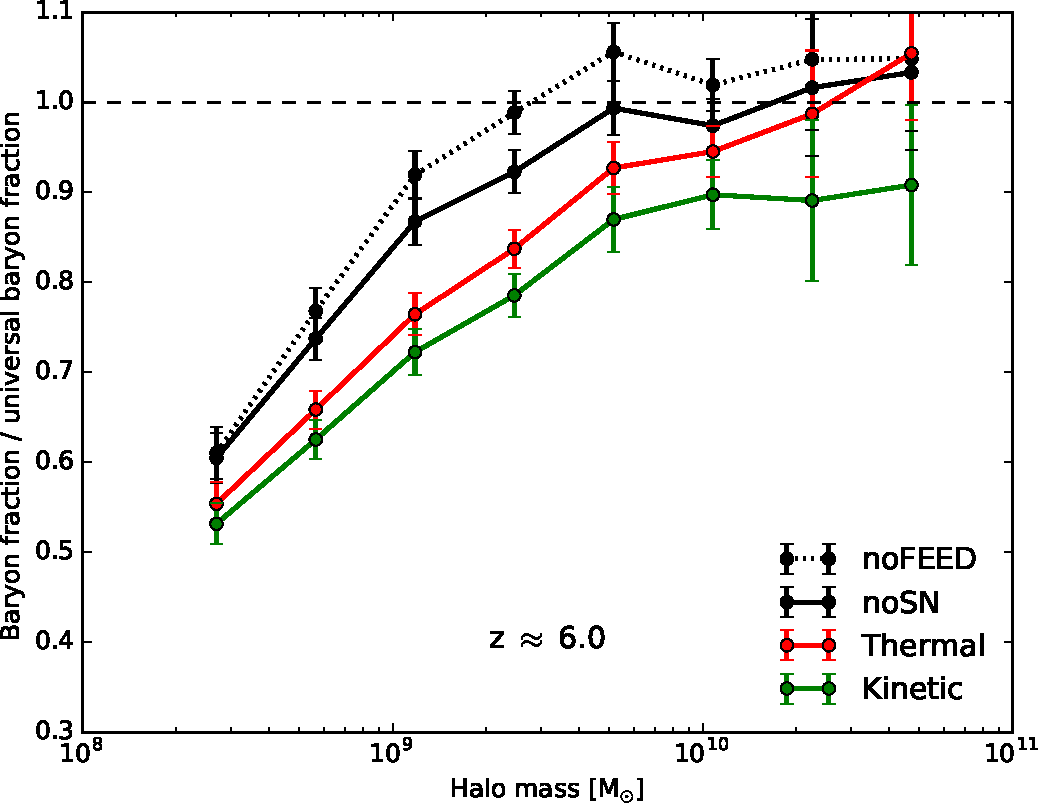
\includegraphics[width=.95\linewidth]{img/03/baryon_frac.pdf}
        \caption[Fraction baryonique]{Fraction baryonique en fonction de la masse du halo et des différentes méthodes de feedback.
 		\label{fig:bfrac}}
\end{figure}


\clearpage
\section{Étude à la surface des halos}

Nous venons d'observer que le feedback de supernovae a un impact sur la composition interne des halos et nous avons interprété ce changement par une expulsion du gaz en dehors des halos.
Nous cherchons ici à quantifier les flux entrants et sortant des halos en fonction de leurs masses.
Je présenterai la méthodologie utilisée pour la détection des flux, ainsi que les résultats obtenus pour les flux hydrodynamiques.
Dans le but de comprendre pourquoi l'histoire d'ionisation n'est pas impactée par le feedback (voir section \ref{sec:pbfesc}), une étude similaire sera réalisée sur les flux radiatifs.
%Une question importante dans l’étude de réionisation est la quantité de rayonnement ionisant sortant des halos.
Nous avons vu que le rayonnement interagit avec les baryons, et nous verrons qu'il existe un liens entre la fraction baryonique déterminée plus haut (sec. \ref{sec:baryon_frac}) et les flux radiatif.

\subsubsection{Healpix}
\label{sec:healpix}

Nous cherchons à déterminer les flux à la surface des halos.
Par soucis de simplicité, nous utiliserons l'approximation du $R_{200}$.
Il faut donc discrétiser la sphère de rayon $R_{200}$ autour de chaque halo.
Cette discrétisation sera réalisée grâce à Healpix \citep{gorski_healpix:_2005}, un outil qui permets de répartir des points de manière uniforme sur la sphere (c.f. figure \ref{fig:HealPix}).
%L'association Healpix/grille sera réalisée par recherche de plus proche voisin 
Par la suite, tous les halos seront discrétisés en utilisant $3072$ points Healpix.
Il est probable, pour les halos les plus petits, qu'une cellule puisse être associée à plusieurs points Healpix.
%L'avantage de cette méthode est que toutes les cellules ont la même pondération.
Comme chaque point Healpix représente une portion constante de la surface de la sphère, la pondération en surface nécessaire pour la gestion des flux, se fait automatiquement.
Une fois la sphère générée, elle sera centrée sur la position du halo, et redimensionnée de telle manière à ce que sa taille corresponde au $R_{200}$ du halo en question.
Puis, pour chaque point de la sphère Healpix, on effectuera une recherche de plus proche voisin à l'aide d'un KD-tree généré sur les centres de cellules, pour déterminer avec qu'elle cellule l'associer.
Nous avons donc accès aux cellules correspondant à la surface du halo.
%Nous connaissons maintenant l'ensemble des cellules au R200 de chaques halos.
Si il est possible de travailler directement avec les grandeurs scalaires, lors d'une analyse vectorielle, les vecteurs seront projetés sur la normale à la sphere.
%Mais nous cherchons a réaliser une étude sur les flux.

%Pour déterminer les flux autours de chaque halo, il est nécessaire de les englober d'une sphère.
%Cette sphère serra discrétisée a l'aide de Healpix (TODO ref) un outils qui permets de répartir des points de manière uniforme sur une surface sphérique .
\begin{figure}
	\centering
    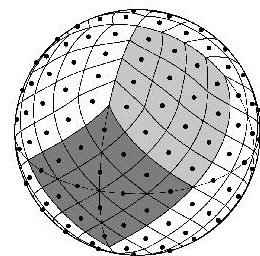
\includegraphics[width=.45\linewidth]{img/03/healpix.jpg} 
    \caption[Sphère HealPix]{Exemple de sphère HealPix. Toutes les cellules sont uniformément réparties et de surfaces identiques.}
 	\label{fig:HealPix}
\end{figure}

\subsection{La vitesse du gaz au $R_{200}$}
\label{sec:snvitesses}

Dans le but de mettre en évidence l'efficacité des supernovae à expulser le gaz des halos, j'ai quantifié la vitesse moyenne du gaz à la surface des halos, au niveau de leur $R_{200}$.
Pour chaque halos, la vitesse moyenne des $3072$ vitesses radiales obtenues est calculée.
Par convention, la normale à la sphère pointe vers l'extérieur, les vitesses positives sont donc sortantes.
Si la vitesse moyenne est positive, le halo perd de la matière baryonique, et sinon il en accrète.
Les figures \ref{fig:R200speed1} et \ref{fig:R200speed2} représentes les résultats obtenus pour les quatre simulations de comparaison.

\begin{figure}
	\centering
	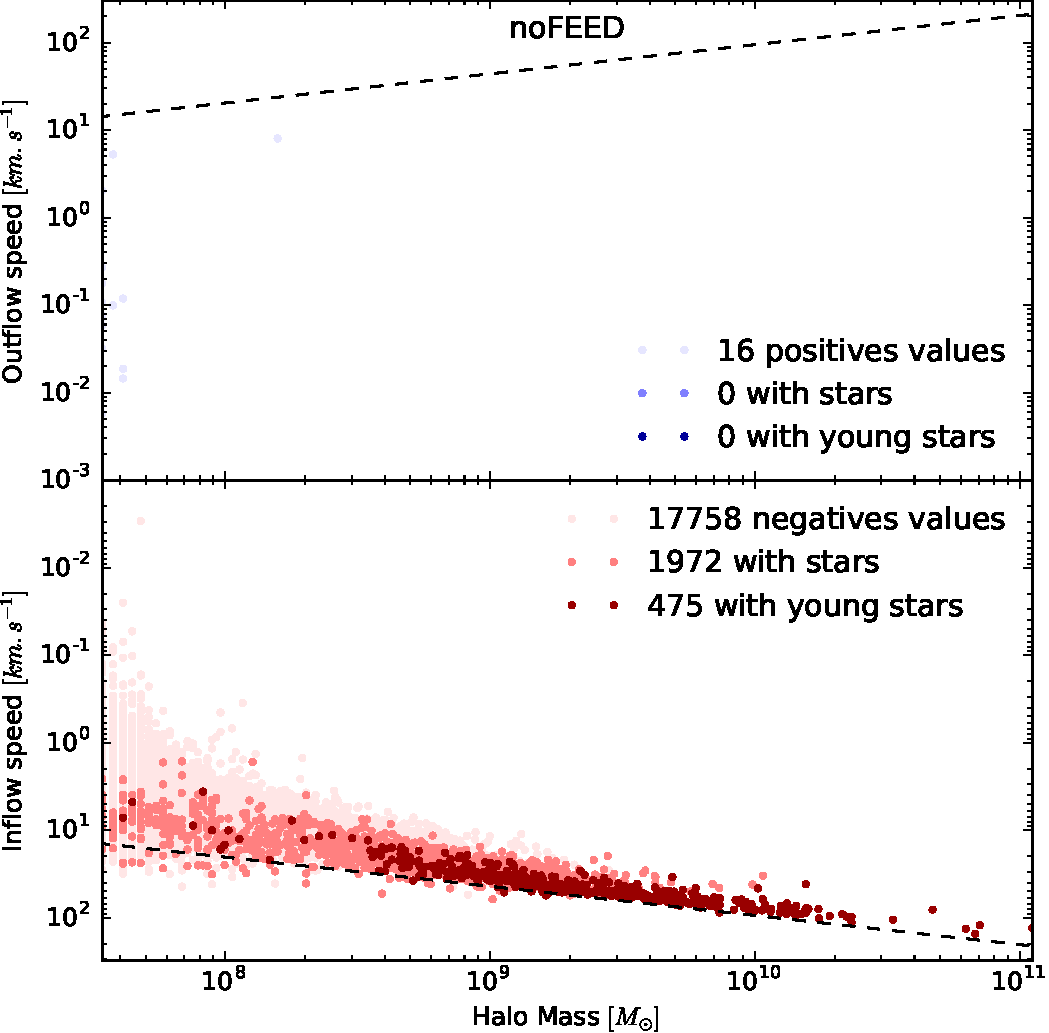
\includegraphics[height=.45\textheight]{img/03/flux_speed_noFEED.pdf} 
	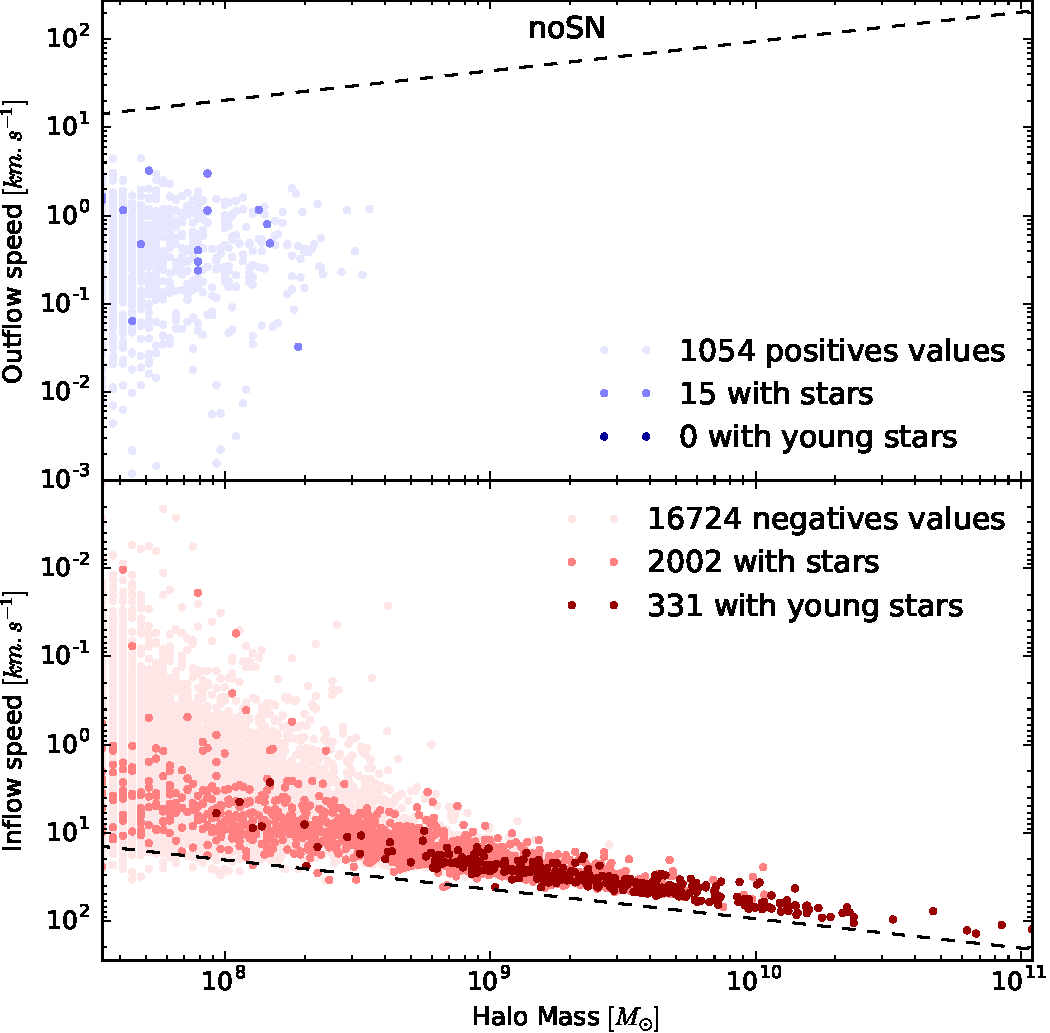
\includegraphics[height=.45\textheight]{img/03/flux_speed_noSN.pdf} 
    \caption[Vitesse du gaz au $R_{200}$ 1]{Vitesse moyenne du gaz au $R_{200}$ en fonction de la masse du halo.
    Les tirets représentent la vitesse de chute libre et d'échappement.
    L'introduction de la radiation fait apparaître des flux sortants aux petites masses.
 	\label{fig:R200speed1}}
\end{figure}

\begin{figure}
	\centering
	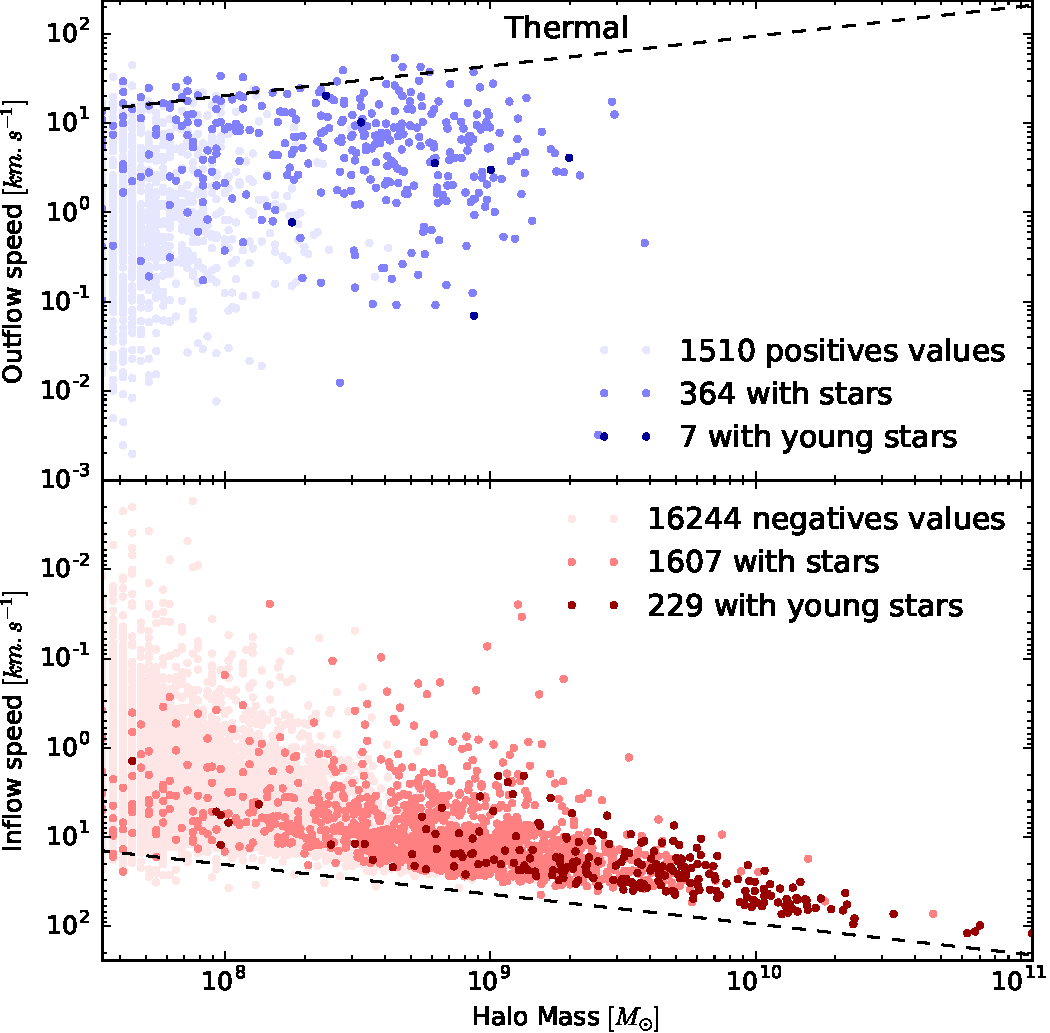
\includegraphics[height=.45\textheight]{img/03/flux_speed_therm.pdf} 
	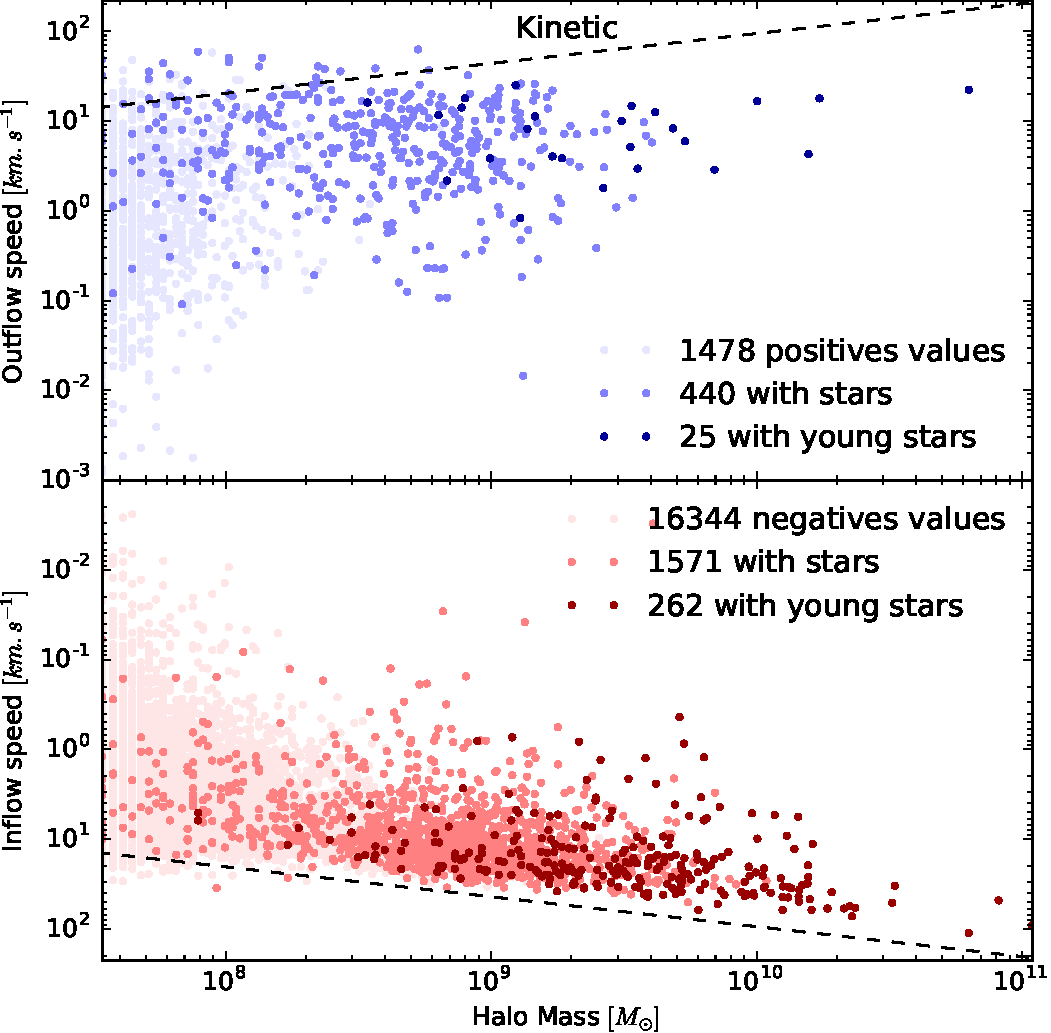
\includegraphics[height=.45\textheight]{img/03/flux_speed_kinetic.pdf} 
    \caption[Vitesse du gaz au $R_{200}$ 2]{Vitesse moyenne du gaz au $R_{200}$ en fonction de la masse du halo.
    Les tirets représentent la vitesse de chute libre et d'échappement.
    L'introduction des supernovæ génère des flux sortants dans une population de halo avec des étoiles veilles (ayant explosées en supernovae).
    Le feedback cinétique est capable de générer des flux sortants pour des halos plus massifs que dans le cas du feedback thermique.
 	\label{fig:R200speed2}}
\end{figure}

Dans le cas idéal, la matière chute sur le halo à la vitesse de chute libre.
A l'inverse, si de la matière est expulsée plus rapidement que cette vitesse limite, elle n'est plus gravitationnellement liée au halo.
Cette vitesse limite est représentée en tirets sur les figures et s'exprime:
\begin{equation}
v_{lim} = \pm \sqrt{\frac{2 GM (r<R_{200})} {R_{200}} } 
\end{equation}

En absence de feedback, la quasi totalité des halos se trouvent sur cette relation limite.
De part la nature collisionnelle des baryons, cette vitesse est une limite supérieure, le gaz accrété étant ralentit par le gaz initialement présent au sein du halo.
Avec l'introduction de la radiation (figure \ref{fig:R200speed1}), il y a apparition d'une population de halos de faibles masses ($M< \mathrm{qq} 10^8 M_\odot$) avec des vitesses moyennes positives.
La radiation est en mesure de générer des flux sortant, et donc de diminuer la fraction baryonique de cette classe de masse. 
Cette population ne possède pas d'étoile, ce qui suggère un effet provenant de l'extérieur des halos, en cohérence avec un photo-chauffage par le rayonnement de halos massifs environnants.
La vitesse d'expulsion moyenne est significativement plus faible que la vitesse d'échappement (1 ou 2 ordres de grandeurs).
Ces flux sortants observés peuvent expliquer la coupure de formation stellaire par le radiation pour les halos de moins $10^9 M_\odot$, observée dans des précédents travaux (eg \cite{ocvirk_cosmic_2015}).

De plus dans la partie accrétante du diagramme on observe que la vitesse limite est globalement plus faible (la population s'est légèrement écartée de la ligne limite).
Le photo-chauffage va limiter l'accrétion par effet thermique, le gaz au centre se dilatant, il oppose plus de résistance à l'effondrement des couches externes.
Également, la dispersion des valeurs moyennes est plus grande, signifiant que la radiation agit sur une large gamme de halos.

Avec l'introduction des supernovae (figure \ref{fig:R200speed2}), il y a apparition d'une nouvelle population dans la partie haute du diagramme.
Cette population possède des étoiles aillant déjà explosées en supernovae, ce qui suggère un effet provenant de l'intérieur.
On observe que les halos possédant des vitesses positives peuvent avoir des masses plus élevées que dans le cas du simple feedback radiatif.
De plus, le feedback cinétique permet de générer des flux sortant sur des halos plus massifs que dans le cas du feedback thermique.
Les vitesses moyennes sont proches de la vitesse d'échappement.
Cependant elles restent quasi toutes, sous la limite de la vitesse de libération.
Dans ces modèles de feedback le gaz est expulsé des halos, mais toujours gravitationnellement lié à eux.

%Dans la littérature, la notion d'\textit{outflows}

\subsection{Le flux radiatif au $R_{200}$}
\label{sec:radflow}

Comme dans ces simulations la lumière est décrite comme une fluide (cf section \autoref{sec:rad_solver}), un travail identique à celui de la section précédente peux être réalisé sur les flux radiatifs.
La figure \ref{fig:R200rad} présente les résultats obtenus.
On observe que seuls les halos avec des étoiles jeunes ont un flux de radiation sortant, que tous les halos de $M>2 \cdot 10^9 M_\odot$ ont un flux radiatif sortant et que le flux est d'autant plus important que ceux ci sont massifs.
Il n'y a pas de différences notables, dans la façon dont la radiation s'échappe des halos, entre les différents types de feedback, 
Cette observation est en accord avec les mesures réalisées en section \ref{sec:pbfesc}, l'évolution de la fraction ionisée ne dépend pas du feedback car la quantité de photon s'échappant des halos ne dépend pas de la méthode de feedback de supernovae.

Les tirets représentes la masse d'un halo ayant un $R_{200}$ de taille équivalente à la résolution radiative.
En effet le transport des photons étant réalisé sur la grille de base (voir section \ref{sec:crta}) la résolution est plus faible que pour l'hydrodynamique.
% car le raffinement n'agit pas sur la radiation.
Il a déjà été observé qu'une partie des halos de moins de quelques $10^9 M_\odot$ voyaient leurs \ac{SFR} impacté par la radiation. %TODO ref
Malheureusement, cette limite en résolution correspond aussi à la taille limite des halos présentant un flux net entrant.
Des simulations à plus hautes résolution sont nécessaires pour déterminer si la limite en flux entrant n'est pas due à un effet de résolution.
Le fait que tous les halos ayant des étoiles jeunes, même en dessous de cette limite, aient un flux sortant (points bleus foncés) est en faveur d'une résolution suffisante. 
De plus, si ce n'était pas le cas, il est probable que l'on ne mesurerai pas une telle continuité dans la tendance.

\begin{figure}
	\centering
	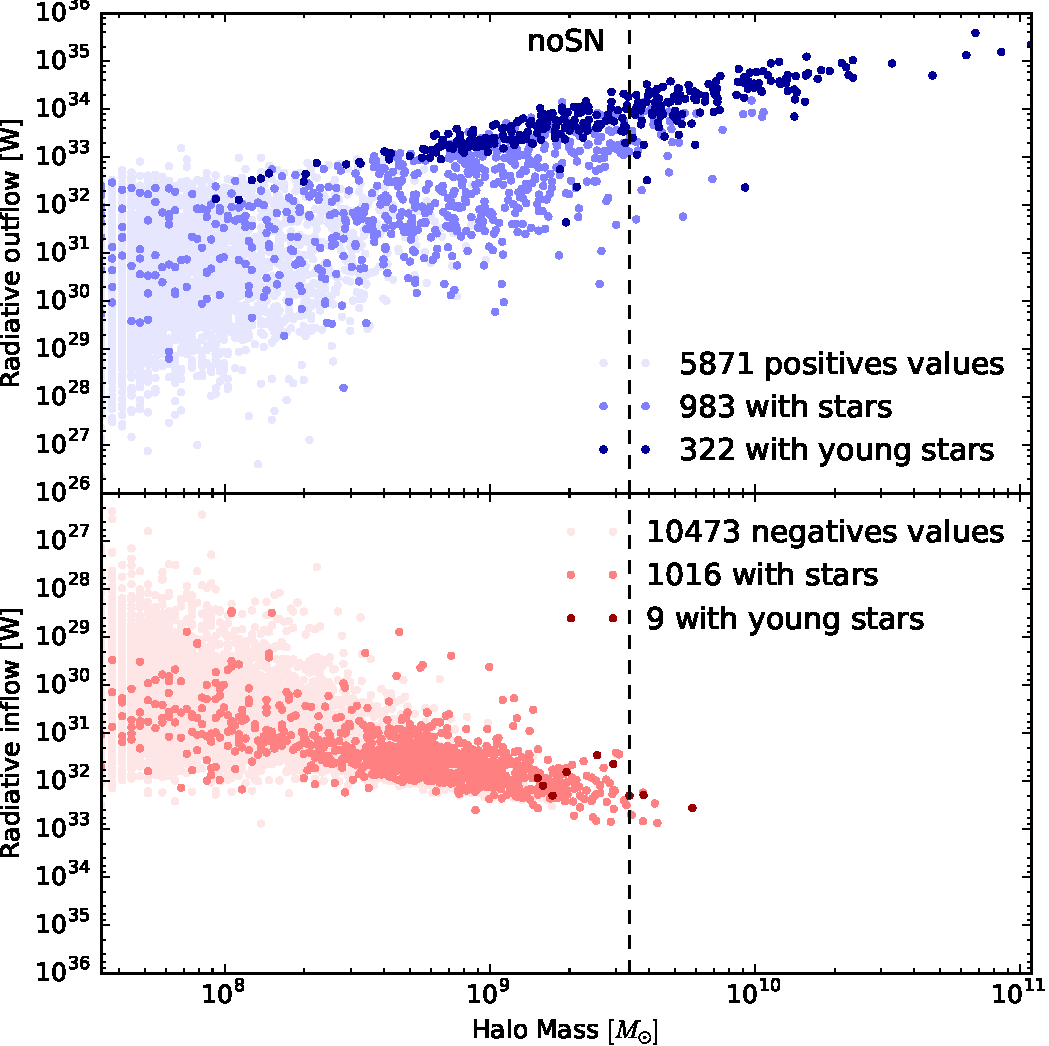
\includegraphics[height=.30\textheight]{img/03/flux_rad_noSN.pdf} 
	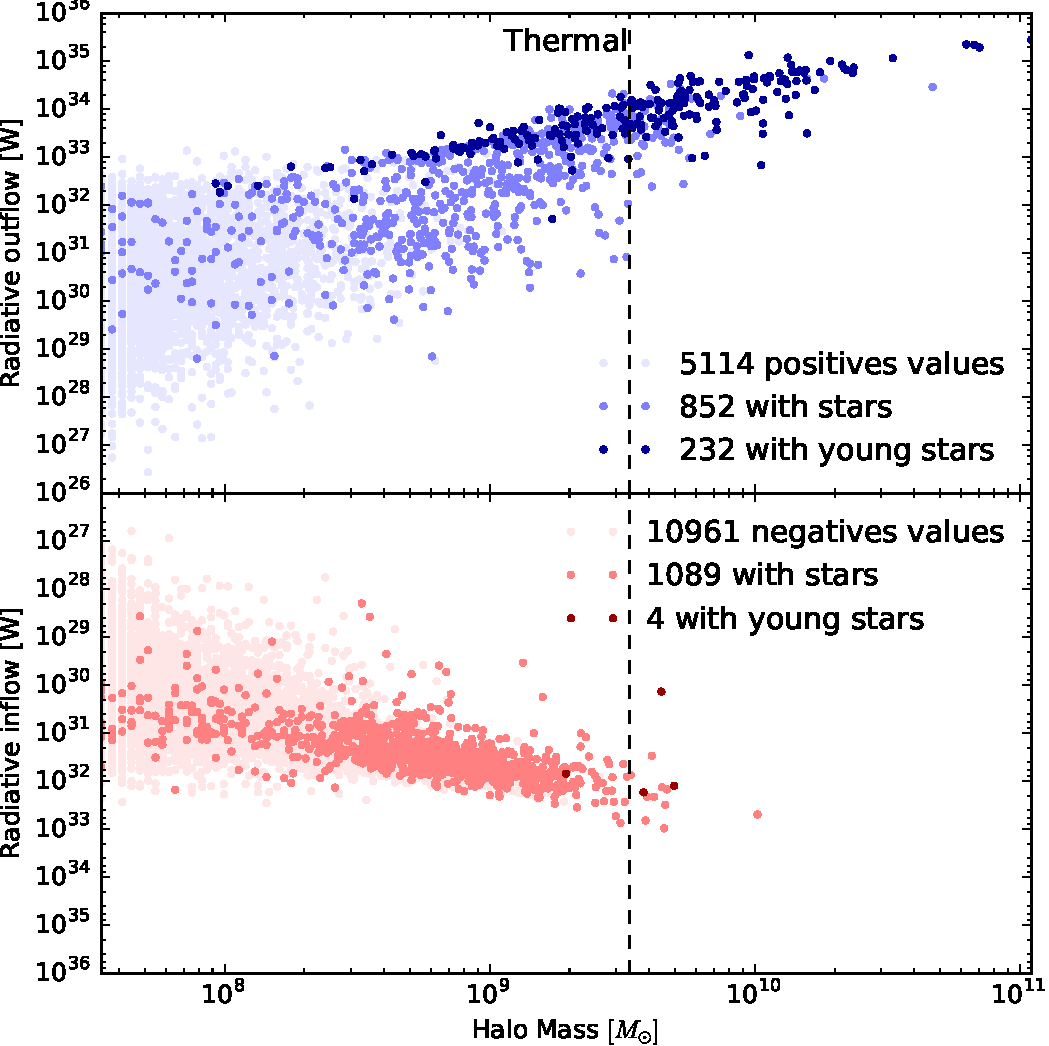
\includegraphics[height=.30\textheight]{img/03/flux_rad_therm.pdf} 
	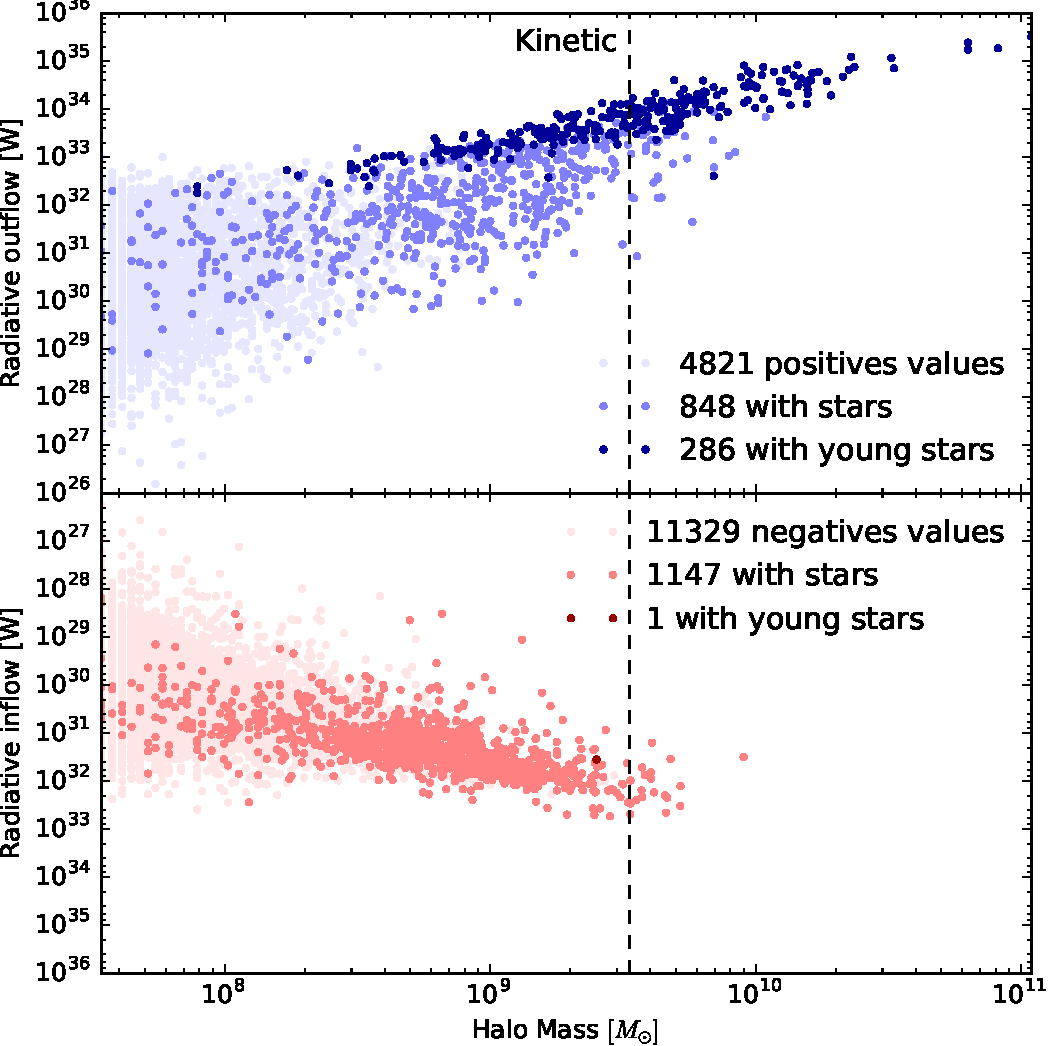
\includegraphics[height=.30\textheight]{img/03/flux_rad_kinetic.pdf} 
    \caption[Flux de photons au $R_{200}$]{Flux de photons au total $R_{200}$ en fonction de la masse du halo. 
    Les halos les plus massifs ont un flux de photons sortant. 
    Une partie des halos les moins massifs ont un flux entrant.}
 	\label{fig:R200rad}
\end{figure}


\subsection{Budget de photons}
\label{sec:photonbudget}
La balance entre les quelques halos massifs émettant beaucoup de photons et les très nombreux halos peu lumineux, est explorée dans cette section.
Connaissant les flux radiatifs des halos, il est possible de déterminer la répartition du budget de photon en fonction de la masse des halos.
L'objectif est de déterminer quels sont les halos qui contribuent le plus à ioniser effectivement l'\ac{IGM} dans les simulations.
La figure \ref{fig:budget} présente les résultats obtenus en faisant la somme des flux sortant de tous les halos d'une certaine classe de masse.
Seuls les flux sortants sont considérés, la calcul est réalisé sur les 3072 points Healpix de tous les halos et non sur les moyennes globales calculées en section \ref{sec:radflow}).
Nous faisons ici la même constatation que précédemment, le budget de photon n'est globalement pas impacté par les supernovae dans nos modèles.
Dans ces simulations, se sont les halos de masses autour de $10^{10} M_\odot$ qui contribuent le plus au budget de photons global.
Il est intéressant de remarquer que cette gamme de masses de halos et représentative des galaxies de type Voie Lactée.
Comme il a été mentionné dans la section \ref{sec:sfr_halo}, cette partie de la \ac{HMF} est à la limite de la convergence, et la taille de ces simulations joue peut être un rôle dans ces conclusion.
Il est possible que dans des simulations plus grandes, disposant de halos plus massifs, le maximum du budget de photon soit décalé vers des masses plus importantes.

\begin{figure}
	\centering
	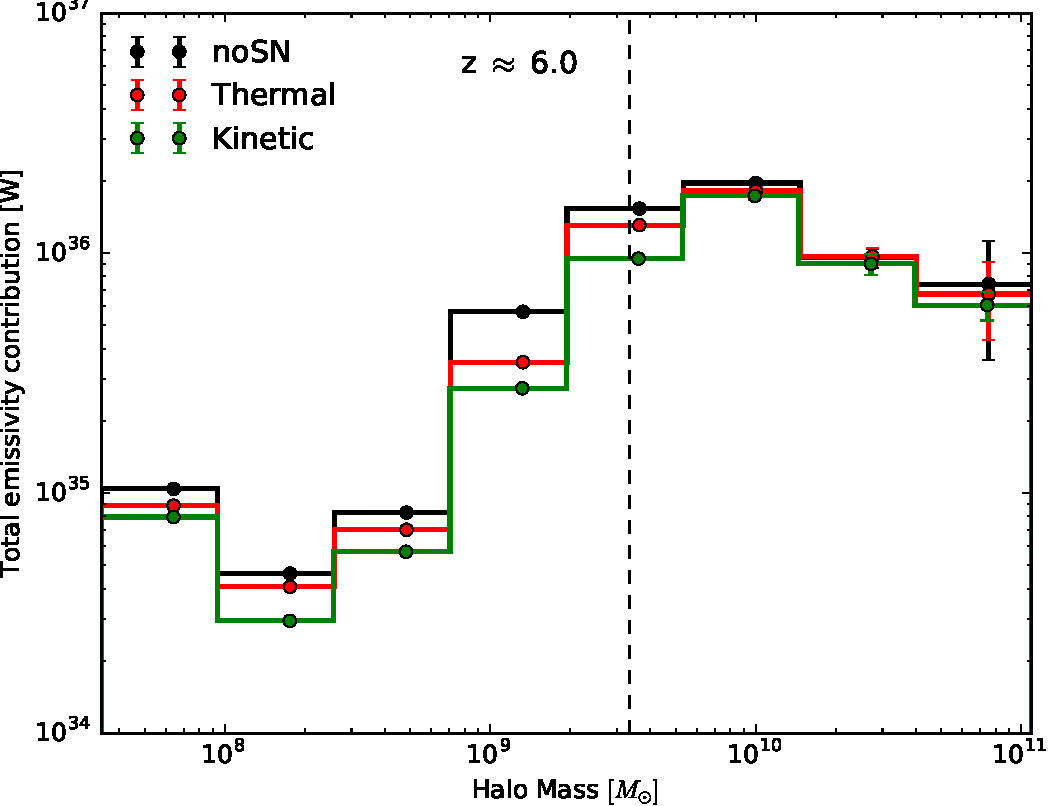
\includegraphics[width=.95\linewidth]{img/03/totout.pdf} 
    \caption[Budget de photon]{Budget de photons en fonction de la masse du halo et du modèle de supernovae. 
    Ce sont les halos de masses autour de $10^{10} M_\odot$ qui contribuent le plus au budget de photons global.
    Les tirets représentes la résolution radiative.
 	\label{fig:budget}}
\end{figure}

\subsection{Fraction d'échappement}
\label{sec:fesc}

En comparant la quantité de photons produite au sein du halo au flux de radiation sortant, il est possible de quantifier une grandeur centrale dans l'étude de la réionisation : la fraction d'échappement des photons $f_{esc}$.
La fraction d'échappement fait le lien entre ce qu'il est possible d'observer et la physique interne au halo.
%Le rapport de la quantité de photon produite sur la quantité de photon sortante, est la fraction d'échappement .
Nous avons vu que le taux de formation stellaire et donc le taux de production de photon, dépend du modèle de supernovae (vois section \ref{sec:sfr_halo}).
Mais nous avons vu que le flux de radiation sortant, lui ne dépend pas du modèle de supernovae.
La fraction d'échappement doit donc varier pour expliquer ce phénomène.
Les $f_{esc}$ obtenues sont présentées sur la figure \ref{fig:fesc}.
Pour compenser le décalage entre le moment d’émission des photons et le moment de leurs passage au $R_{200}$.
Les émissivités sont corrigées du temps nécessaire au parcours des photons entre le centre du halo et son $R_{200}$ \citep{kimm_feedback-regulated_2017}.
\begin{equation}
f_{esc} = \frac{ F_{200}} {\sum \dot{N}_{\left( t-\frac{R_{200}}{\tilde{c} } \right) } }.
\end{equation}
Pour les halos en dessous de la limite en résolution radiative (cf section \ref{sec:radflow}) l'interprétation est difficile, mais il semble que la $f_{esc}$ ne dépende pas du modèle de supernovae.

On mesure une nette augmentation de la fraction d'échappement pour les halos massifs, lors de l'introduction de supernovae cinétique.
En effet, comme le flux radiatif sortant des halos ne semble pas impacté par le feedback (cf section \ref{sec:radflow}) mais que la production interne est significativement réduite (cf section\ref{sec:sfr_halo}), le fraction d'échappement ne peut qu'augmenter.

\begin{figure}
	\centering
	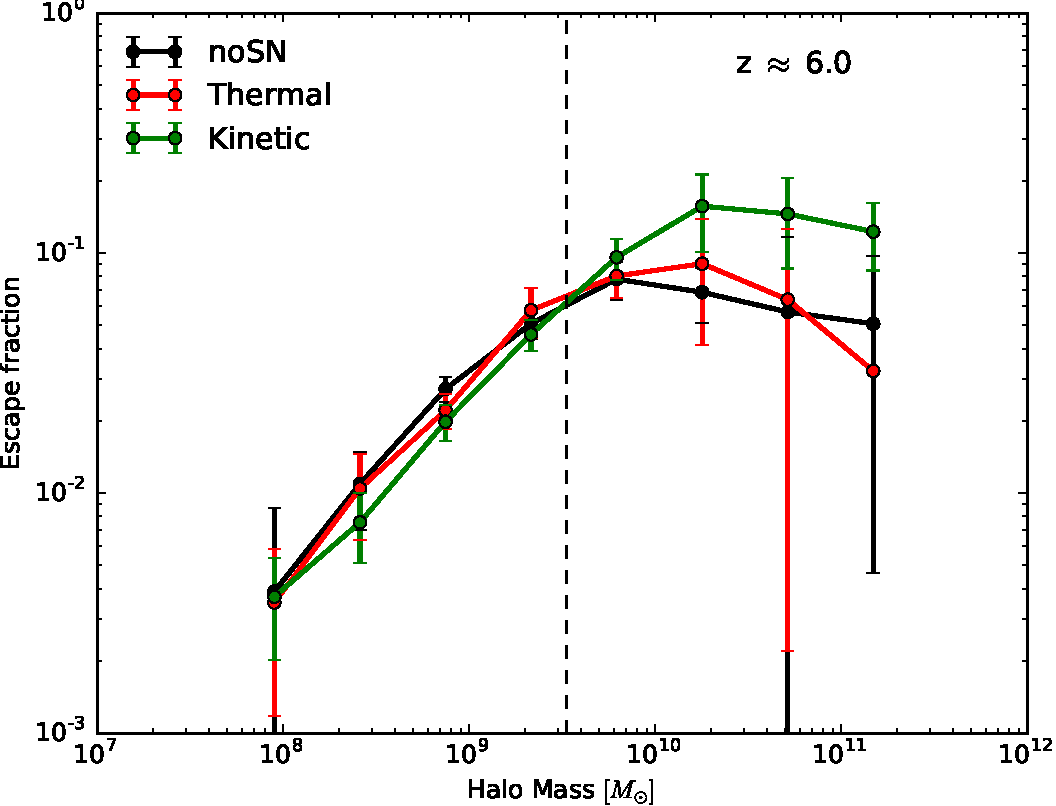
\includegraphics[width=.95\linewidth]{img/03/fesc.pdf} 
    \caption[Fraction d'échappement des photons]{Fraction d'échappement des photons en fonction de la masse du halo et du modèle de supernovae.
    Le modèle cinétique augmente significativement la fraction d'échappement des photons.
    Les tirets représentes la résolution radiative.
 	\label{fig:fesc}}
\end{figure}


\section{Conclusion}
%fonction de luminosité 

Nous avons comparé dans cette partie deux méthodes pour gérer les supernovae dans les simulations cosmologique.
L'objectif est de réaliser des simulations de type échantillons, dans le but de mieux cerner les processus actifs dans les simulations plus grandes de type CoDa.
Nous avons vu (sections \ref{sec:snmethod} et \ref{sec:snegy}) que la formation stellaire est fortement couplée à la méthode et à la quantité d'énergie injectée.
Une injection d'énergie sous forme cinétique sera plus efficace pour réguler la formation stellaire qu'une méthode par injection thermique, et plus la quantité d'énergie injectée sera élevée, meilleure sera la régulation.
La formation stellaire ne dépend que de la quantité de gaz présent dans la cellule (section \ref{sec:schmidt-kennicut}).
Sa régulation se fait par l'intermédiaire de l'expulsion des baryons des halos, qui est visible sur les cartes de champs (section \ref{sec:snmaps}), au sein des halos (section \ref{sec:baryon_frac}) et au niveau du $R_{200}$ (section \ref{sec:snvitesses}), privant ainsi les zone de formation stellaire de matière première.
Comme se sont les particules stellaires jeunes qui émettent du rayonnement ionisant (section \ref{sec:etoilerad}), la formation stellaire est directement liée a la quantité de radiation produite au sein des halos.
La production de photons est réduite en même temps que le \ac{SFR}.
En ayant moins de photons produit, le milieu devrait ioniser moins vite, ce qui devrait être visible sur l'évolution de la fraction d'ionisation.
Or nous avons observé en section \ref{sec:pbfesc} que ce n'est pas le cas, l'histoire d'ionisation est presque indépendante de la méthode d'injection d'énergie de supernovae, alors que le budget de photon lui est impacté.
Nous avons expliqué cet effet en observant que les flux de radiation à la surface des halos ne semble pas impactés par le modèle d'injection d'énergie (section \ref{sec:radflow}).
Dans le cas du feedback cinétique, comme le flux sortant est inchangé alors que la production interne diminue, la fraction d'échappement augmente (section \ref{sec:fesc}).

Au final cette augmentation de la fraction d'échappement peut être expliquée par la diminution de la fraction baryonique.
En effet, comme la \ac{HMF} n'est pas impactée par le feedback (section \ref{sec:hmf}), la quantité de baryon dans les halos diminue avec l'introduction de supernovae.
Or, cette diminution de la quantité de baryon, permet à la radiation de s'échapper plus facilement.

Aux résolutions considérées dans cette étude, c'est a dire la résolution des plus grosses simulations de la réionisation de type CODA,  %TODO ref.
la compétition entre la diminution du taux de production de photon et l'augmentation de la fraction d'échappement semble neutre.
De plus, plus les supernovae sont puissantes, plus le pas de temps est réduit, et plus le coût global de la simulation augmente.

Si une telle simulation est exécutée dans le but d'étudier l'état d'ionisation de l'\ac{IGM}, l'introduction des supernovae n'est pas fondamentale puisqu'elle n'a que peu d'influence sur ce facteur.
A l'inverse, si l’intérêt est plus porté sur la morphologie des galaxies pendant la réionisation, il n'est plus possible de se passer de l'introduction du feedback, car la distribution des baryons au sein des halos peut être grandement influencée.

%De plus nous observons que le budget de photons est principalement gouverné par les halos de masses intermédiaire autour de $10^{10} M_\odot$.

Un changement de comportement dans la formation stellaire est attendu autour de $M \approx 10^9M_\odot$ (voir eg \cite{2001PhR...349..125B}).
La résolution des simulations actuelles n'est pas suffisante et il me semble nécessaire d'augmenter la résolution en masse ainsi que la résolution radiative de un voir deux ordres de grandeurs, pour résoudre la physique des halos jusqu'à des masses de l'ordre de $M \approx 10^8M_\odot$ et ainsi étudier ce changement de régime de manière plus assuré, tout en gardant un volume simulé suffisamment grand.
Quelques années seront encore nécessaire pour réunir ces conditions.
%à la fois une résolution radiative suffisante et .







